\documentclass{anstrans}

\usepackage{url}
\usepackage{multirow}
\usepackage{subfigure}
%%%%%%%%%%%%%%%%%%%%%%%%%%%%%%%%%%%
\title{Modernizing Computational Nuclear Engineering Education in the Open}
\author{Kathryn~Huff$^{1}$, Anthony~M.~Scopatz$^{2}$}
\institute{
$^{1}$ The University of California -- Berkeley, Berkeley, CA 94709 \\
\and $^{2}$ The University of South Carolina, Columbia, SC 29208 \\
}

\email{huff@berkeley.edu}

%%%% packages and definitions (optional)
\usepackage{graphicx}

% allows inclusion of graphics
\usepackage{booktabs}

% nice rules (thick lines) for tables
\usepackage{microtype}

% improves typography for PDF
\newcommand{\SN}{S$_N$}
\renewcommand{\vec}[1]{\bm{#1}}

%vector is bold italic
\newcommand{\vd}{\bm{\cdot}}

% slightly bold vector dot
\newcommand{\grad}{\vec{\nabla}}

% gradient
\newcommand{\ud}{\mathop{}\!\mathrm{d}}

\begin{document}

%%%%%%%%%%%%%%%%%%%%%%%%%%%%%%%%%%%%%%%%%%%%%%%%%%%%%%%%%%%%%%%%%%%%%%%%%%%%%%%%
\section{Introduction}

In the very early days of computing, nuclear engineering applications drove the
majority of innovation in computers, computation, and scientific simulation
\cite{rhodes_making_2012}. Today's nuclear engineering students, however, are
not poised to become leaders in computing, as was once the case. Modern
scientific computing best practices have the potential to revitalize research
computing in our domain and provide broader opportunities in industry for
graduating students. But first, we must teach those practices to the next
generation of nuclear engineers.

We present an example course syllabus that will introduce university students
to modern computational concepts and tools. By incorporating recent insights
from software development, this course equips students with skills essential
to effective research in the data- and computing- intensive domain of nuclear
engineering.  To transform students into more effective researchers, this
course emphasizes:

\begin{itemize}
\item \textbf{Accessibility}: with a contemporary, high-level, object-oriented, open-source programming language,
\item \textbf{Power}: with sophisticated library design principles and powerful data structures,
\item \textbf{Accuracy}: with workflows that emphasize testing and capture provenance,
\item \textbf{Openness}: with projects and exercises emphasizing open science, code review, and collaboration.
\end{itemize}

In this way, the course follows the topics in the book, ``Effective Computation
in Physics: A Field Guide to Research in Python'' \cite{scopatz_effective_2015}
and uses that work as the course textbook.  By emphasizing projects along the
way, the students in this course will learn to create free and open source
tools, verify the functioning of those tools, and publish them online.
Additionally, the syllabus for this course is open-source licensed, allowing
professors to use, re-mix, and collaboratively improve the syllabus for free.

This summary will first motivate the need for new university-level nuclear
engineering  computational curriculum  from the perspective of  scientific
software development and data analysis best practices.  Next, this summary will
introduce the project-driven content and timeline for the course as well as the
collaborative nature of lesson content itself. Finally, the success of
similar training will be discussed along with a schedule of future pilots of
the course.

\section{Motivation and Strategy}

% nuclear engineering used to be at the top
%% we have enormous data
%% we used to drive research

% by failing to keep up, we've fallen behind
%% we still use fortran
%% we don't revamp our computational classes accordingly

% other domains are incorporating data science and modern software methods
%% in doing so, they are able to uncover new insights in their domains
%% we can too

% as it stands students leave unready to contribute to research
%% efficient use of computers is efficient science
%% incorporating the school-of-open-source into the curriculum alleviates this

Nuclear engineering once led the world in computing and has fallen behind, but
not because our computing challenges have gotten easier. In fact, nuclear engineering
applications continue to rely on enormous datasets in many dimensions, traverse
disparate scales, incorporate many physics, and demand precision.

For example, the driving equation for neutron behavior, the time-dependent
Boltzmann equation, is solved in a 7-dimensional phase space, ($3$ in space, $2$
in angle, and one each in energy and time). The scale of a nuclear reactor
simulation is therefore inherently large, spanning five orders of magnitude in space and
ten in neutron energy. Resolved discretization across those scales would require
over $10^{17}$ degrees of freedom per timestep, well beyond the
capabilities of even exascale computing. In this way, without sophisticated
data and analysis methods, we would run out of computational resources before
heat transport, fluid flow, or material performance in the reactor had even
been addressed.

Faced with data and simulation scales such as these, it is imperative
that nuclear engineering students are prepared to reclaim a leadership role in
cutting edge scientific computation. Equipping the next generation of
students with effective computational skills will certainly lead to breakthrough
advancements in nuclear engineering research and development.
Specifically, training them in best practices already commonplace in commercial
software development could have an enormous impact on reproducibility in
nuclear science and engineering. Thus equipped, their contributions to nuclear
engineering may even have a revitalizing effect on the field.

\subsection{Python as a First Language}

One explanation for technological stagnation in our courework might be our
historic reliance on legacy code. In nuclear engineering, the regularoty climate
has has necessitated the use of battle-hardened software implemented in legacy
programming languages. Accordingly, contemporary programming languages are
absent from our curriculum, and so too are the best practices in scientific
software development \cite{wilson_best_2014} that have evolved alongside them.

Specifically, due to our reliance on legacy software written in Fortran, the
undergraduate first course in computing at many Nuclear Engineering departments
emphasize MATLAB or Fortran rather the contemporary equivalents, Python and C++.

Python, a high-level, dynamically-typed language, is now the most popular
language for inroductory Computer Science curriculum \cite{guo_python_2014} and
is very popular for education more broadly
\cite{myers_python_2007,stajano_python_2000,backer_computational_2007}. Its
readable syntax \cite{stefik_empirical_2013}, straightforwared
object-orientation, and open source packages give it an enormous educational
advantage over competitors (see Figure \ref{fig:guo}) whose licenses limit the
flexibility and shareability of software produced within those frameworks.

\begin{figure}[htbp!]
\begin{center}
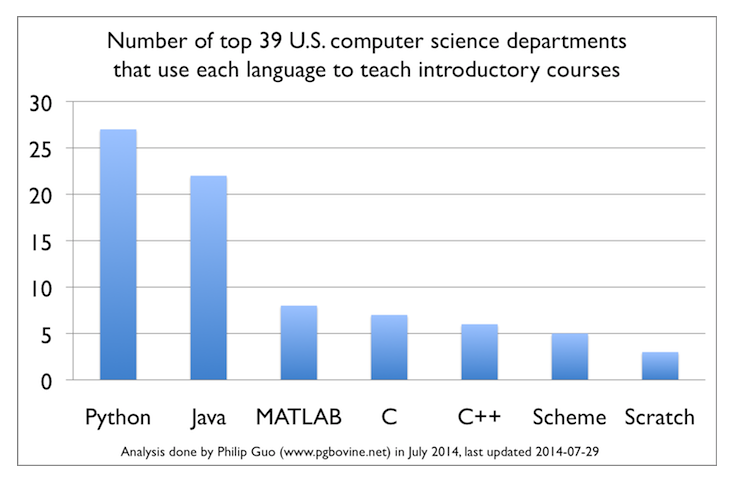
\includegraphics[width=0.4\textwidth]{guo.eps}
\end{center}
\caption{Python popularity in introductory computer science curriculum. Figure
reproduced from \cite{guo_python_2014}. }
\label{fig:guo}
\end{figure}


In addition to the above reasons, the authors recommend using Python
because object-orientated languages are already becoming common in nuclear
engineering software development.  Neglecting object orientation at the high
level (with MATLAB) or at the low level (with historical Fortran) leaves students
unprepared to participate in the cutting edge software in our field,
increasingly written in those object oriented languages (e.g.
Serpent\cite{leppanen_serpentcontinuous-energy_2013}, 
MOOSE\cite{gaston_moose:_2009}, and
PyNE\cite{scopatz_pyne:_2012}). It should be noted that modern Fortran specifications 
are object-oriented.  However, these capabilities are often not covered in 
engineering courses in favor of a more long-standing procedural style from historical
Fortran languages.


\subsection{Efficient and Reproducible Workflows}

Best practices for efficient and reproducible modeling and analysis, though
common in commercial software development, are typically missing from nuclear
engineering curriculum as well. A similar lack of such workflows across
academic science at large and is  at the root of an enormous credibility
crisis in scientific computing \cite{donoho_reproducible_2009,
stodden_scientific_2010}.

Tools available for reproducible science should be emphasized early in order to
prepare students for the rigor of engineering work. Concepts such as
verification and validation should be instilled in a computational course.
Doing this through the implementation of unit test suites, version control,
debugging skills, and other defensive programming techniques will create
more accurate and reliable software.

\subsection{Open Source and Open Science}

Computational tools and data grow more robust with a broad base of users and
developers \cite{petre_code_2014, wicherts_willingness_2011}. The physics
community has used this fact to the great benefit of, for example, the Large
Hadron Collider experiment. In that instance, faced with an enormous computing
challenge and potential for human error, the experimenters opened both the
software and the data to the whole world. This massive scale peer review is
unknown in nuclear where a combination of export control issues and antiquated
workflow paradigms mean that only a very small number of tools have been open
sourced \cite{gaston_moose:_2009}\cite{scopatz_pyne:_2012}\cite{carlsen_cyclus_2014}.

In addition for formulating the course around an open source language (Python),
the projects in the course are focused on student contributions to actual open source
projects in nuclear engineering. Potential code-bases to which studnets could
propose contributions include MOOSE\cite{gaston_moose:_2009},
PyNE\cite{scopatz_pyne:_2012}, \textsc{Cyclus}\cite{carlsen_cyclus_2014}, and
even OpenMC\cite{romano_openmc_2013} and OpenMOC\cite{boyd_openmoc_2014}.

The skills learned in contributing to open source software go far beyond best
practices in computing. They extend to the skills needed for scientific
collaboration including communication, peer review, and objectivity.

\subsection{Example Syllabus}

To train the workforce in a authors recommend a course covering the topics
above in a high level language (Python). A twelve week course with two days per
week would have the following schedule:

\begin{table*}[t]
\centering
\begin{tabular}{|l|r|l|r|}
\hline
\textbf{Part} & \textbf{Lesson} & \textbf{Content} & \textbf{Project} \\
\hline
\multirow{6}{*}{\textbf{Getting Started}}
& 1 & Introduction to the Command Line
& \multirow{6}{*}{\textbf{Fuel Geometry Class}}\\
& 2 & Programming Blast Off with Python & \\
& 3 & Essential Containers & \\
& 4 & Flow Control \& Logic & \\
& 5 & Operating with Functions & \\
& 6 & Classes and Objects & \\
\hline
\multirow{6}{*}{\textbf{Getting It Done}}
& 7 & Regular Expressions
& \multirow{6}{*}{\textbf{Database I/O and Visualization}}\\
& 8 & NumPy: Thinking in Arrays & \\
& 9 & Storing Data: Files \& HDF5 & \\
& 10 & Important Data Structures & \\
& 11 & Analysis and Visualization & \\
& 12 & Performing in Parallel & \\
\hline
\multirow{6}{*}{\textbf{Getting It Right}}
& 13 & Deploying Software
& \multirow{6}{*}{\textbf{Continuously Integrated Test Suite}}\\
& 14 & Building Software Pipelines & \\
& 15 & Local Version Control & \\
& 16 & Remote Version Control & \\
& 17 & Debugging & \\
& 18 & Testing & \\
\hline
\multirow{4}{*}{\textbf{Getting It Out There}}
& 19 & Automated Documentation
& \multirow{4}{*}{\textbf{Reproducible Publication}}\\
& 20 & LaTeX & \\
& 21 & Collaboration Tools& \\
& 22 & Licenses, Ownership, and Copyright & \\
\hline
\end{tabular}
\caption{Lesson content per week.}
\label{tab:syllabus}
\end{table*}


The syllabus above, along with lesson plans, exercises, customizable homeworks,
grading rubrics, and project assignments is to be released online by Fall 2016.
The syllabus is also an open and collaborative resource, which can be used
and modified freely.

\subsection{Textbook: Effective Computation In Physics}

\begin{figure}[htbp!]
\begin{center}
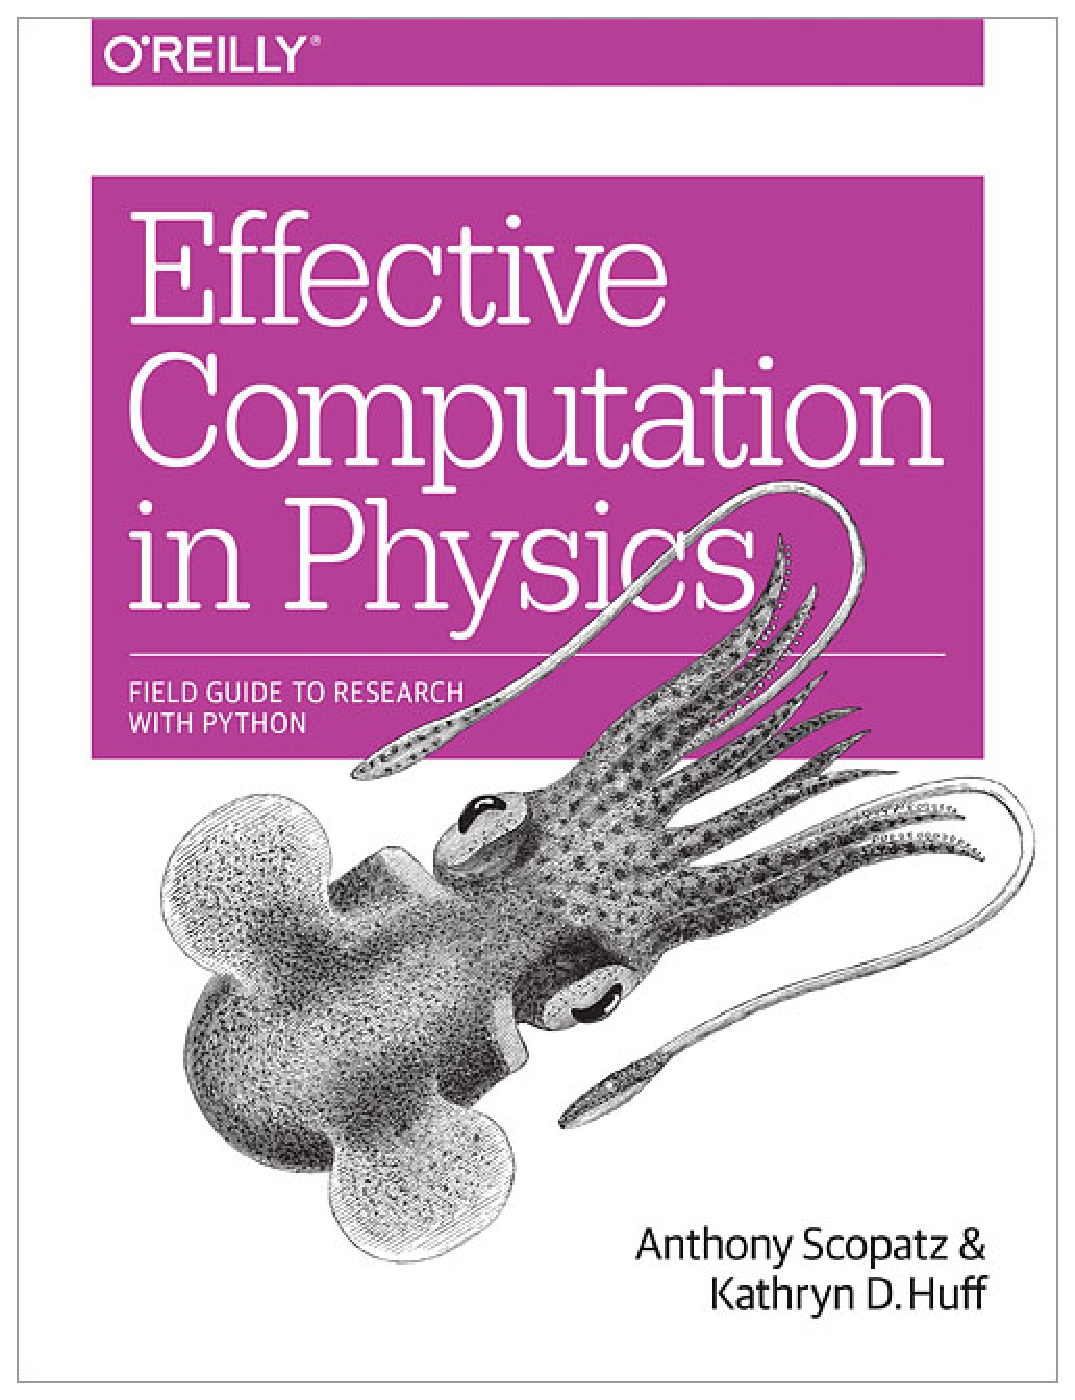
\includegraphics[width=0.4\textwidth]{ecip.eps}
\end{center}
\caption{The textbook for the course is Effective Computation in Physics: A Field Guide To Research in Python}
\label{fig:book}
\end{figure}

The textbook.


\section{Experience}

Similar approaches have produced positive outcomes in courses within other domains
(e.g. biology 
\cite{matthews_using_2010,honts_evolving_2003,tjaden_multidisciplinary_2007,libeskind-hadas_first_2013} 
and physics\cite{baxter_scientific_2014,myers_python_2007}) and have as workshop-style  
\cite{huff_rapid_2011,wilson_software_2006,wilson_software_2014}

\subsection{Software Carpentry}

The material and concepts proposed here were heavily influence by the work done
by the Software Carpentry Foundation, an organization that

Software Carpentry has been involved with teaching scientific computing best
practices for over a decade. Students have come from many areas of science and
usually no programming experience is necessary to attend a course. The courses
are typically two days and cover skills for "Doing more with less pain."

Also, the testing, debugging, and collaboration sessions were taught as a part
of a recent workshop at the University of California Berkeley. The students, in
the course of four hours, were able to upload tests and example code to a
version controlled repository and to deploy continuous integration for
automated unit testing.

\section{Conclusions}

This course will equip students with contemporary concepts that will make them more
effective researchers in the data and computing intensive domain of nuclear
engineering. The course prepares students with fundamental skills such
as mobility in the UNIX shell, scripting, analysis, and visualization. Beyond
that, it prepares them for more high performance computing tasks by introducing
object orientation, databases, and parallelization. It also prepares them to
incorporate reproducibility and accuracy into their scientific work through
version control, testing, and automated workflow pipelines.  Finally, by
emphasizing the contributions to real open source projects along the way, the
students in this course will learn to create and collaborate on free and open
source tools, verify the functioning of those tools, and publish them online.
Finally, the syllabus and course textbook are open and affordable,
respectively.

%%%%%%%%%%%%%%%%%%%%%%%%%%%%%%%%%%%%%%%%%%%%%%%%%%%%%%%%%%%%%%%%%%%%%%%%%%%%%%%%
%%%%%%%%%%%%%%%%%%%%%%%%%%%%%%%%%%%%%%%%%%%%%%%%%%%%%%%%%%%%%%%%%%%%%%%%%%%%%%%%
\bibliographystyle{ans}
\bibliography{bibliography} \end{document}
